\providecommand{\main}{../../../..}
\documentclass[\main/dresen_thesis.tex]{subfiles}

\begin{document}
  \begin{figure}[tb]
    \centering
    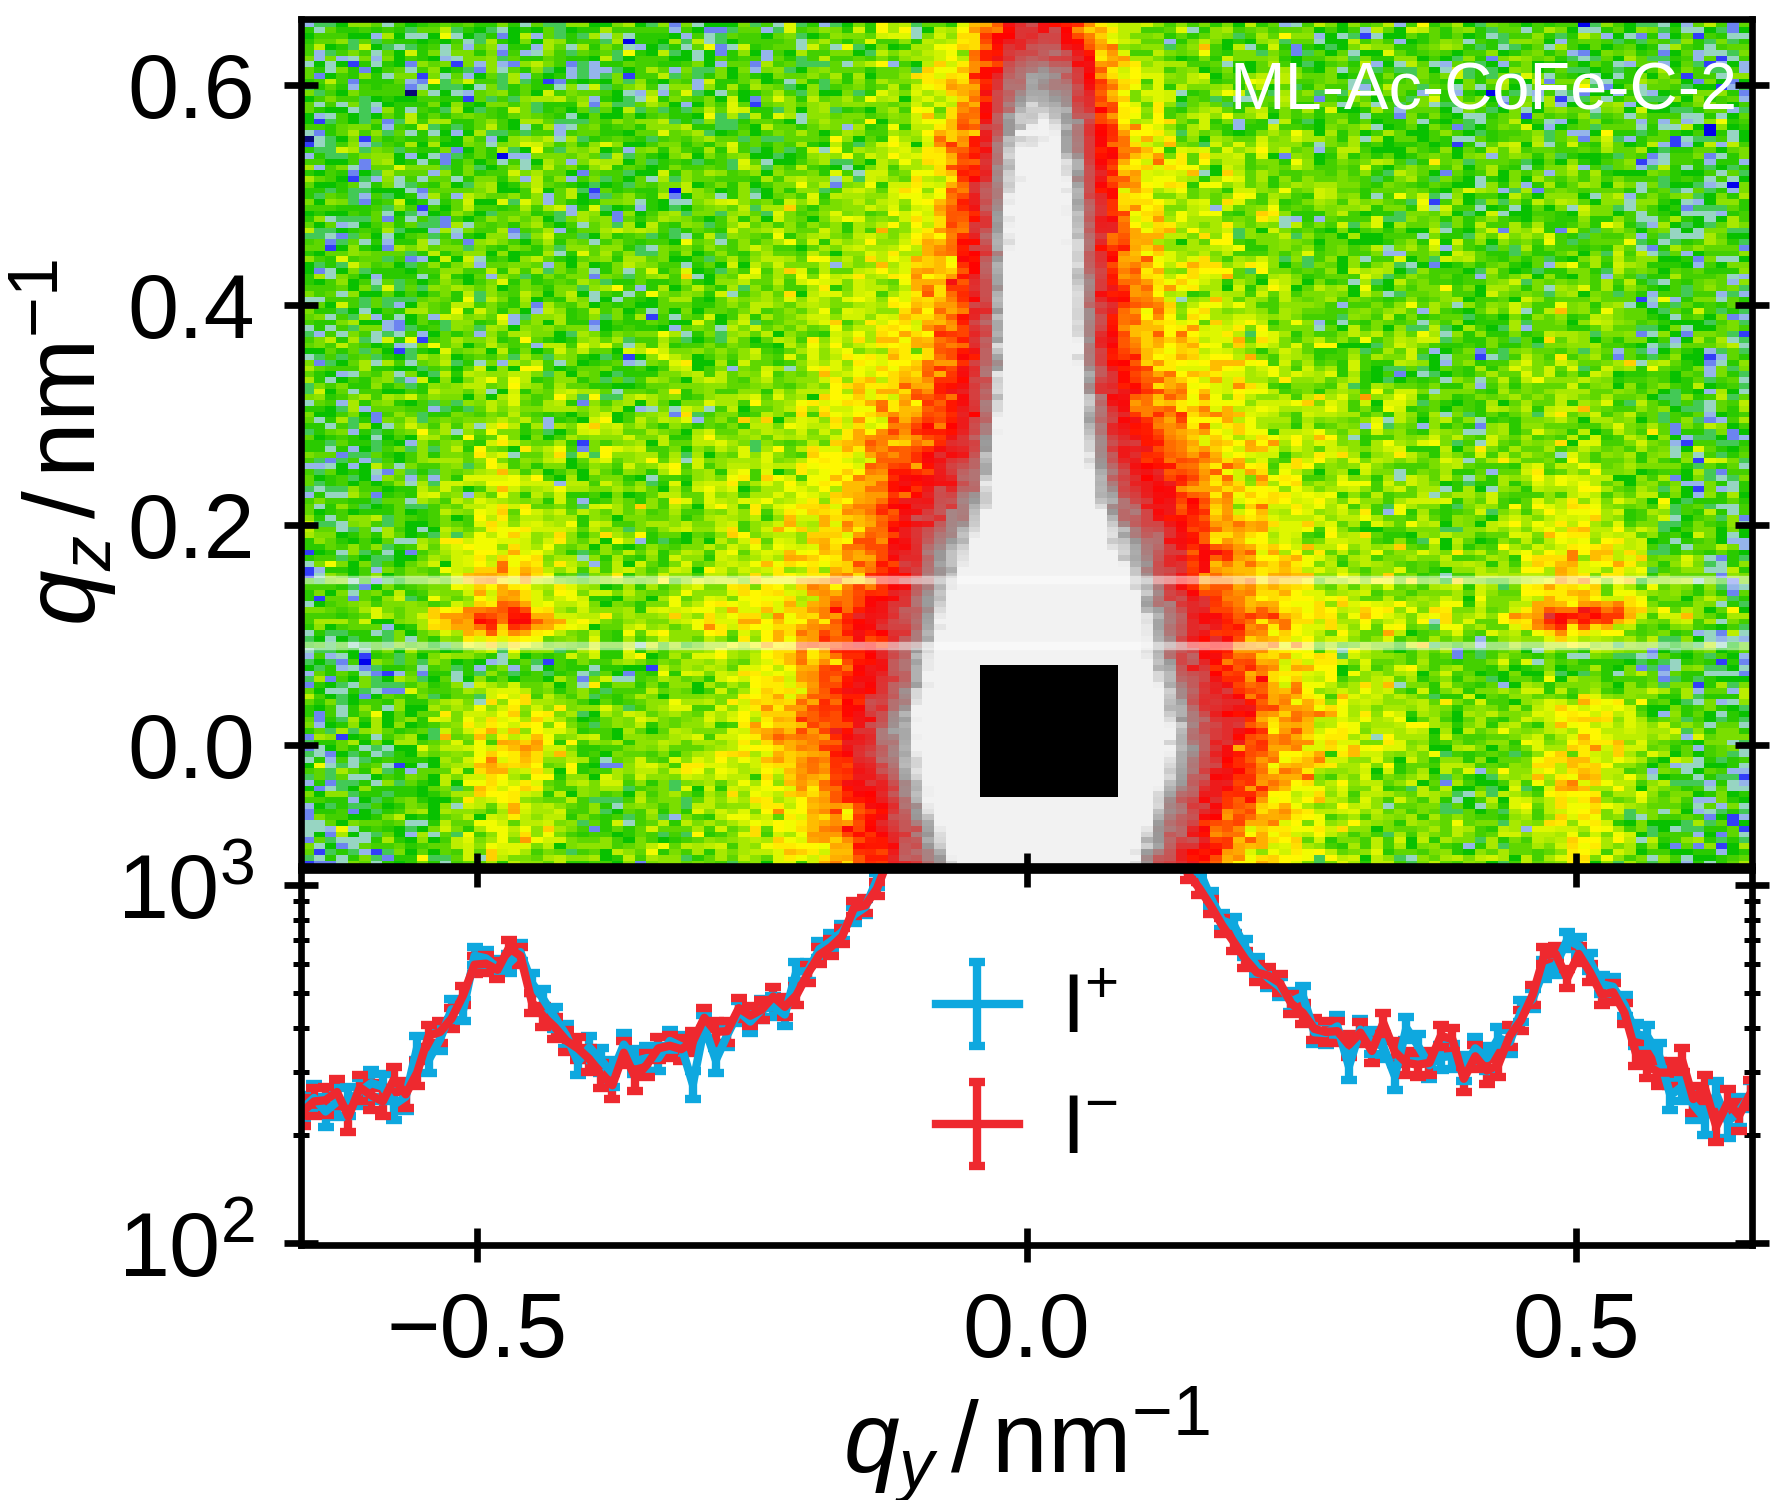
\includegraphics{monolayers_GISANS_ML-Ac-CoFe-C-2_ZFC5K_GF}
    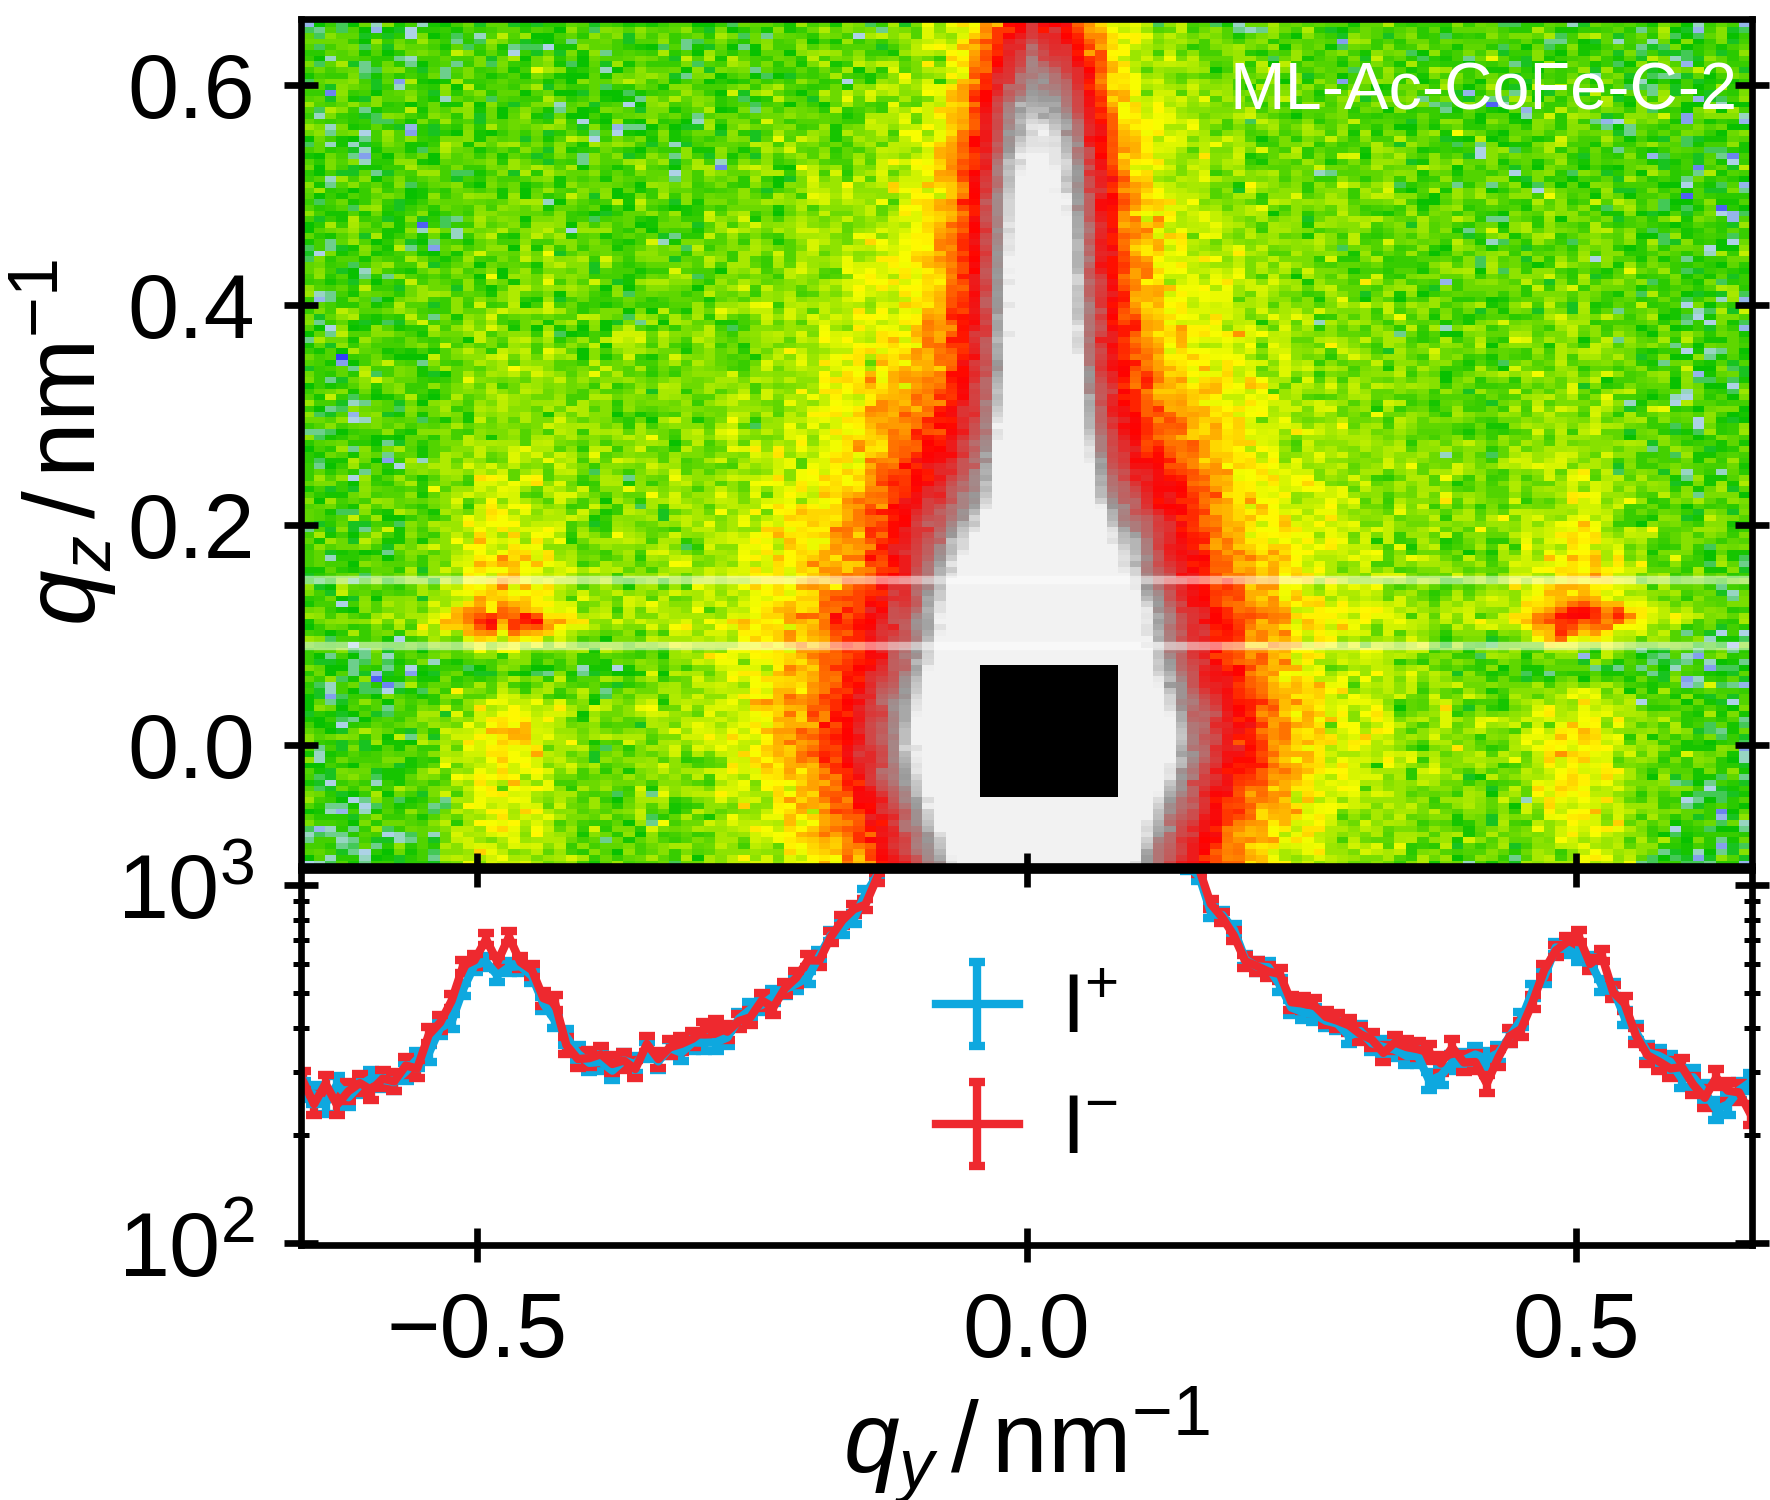
\includegraphics{monolayers_GISANS_ML-Ac-CoFe-C-2_ZFC5K_Remanence}
    \caption{\label{fig:monolayer:magneticStructure:polGisans5KZFC}Polarized grazing-incidence small-angle neutron scattering of ML-Ac-CoFe-C-2 after zero-field cooling to $5 \unit{K}$. Left is the detector image $I^{+}$ measured at guide field ($5 \unit{mT}$) after zero-field cooling and right the detector image of $I^{+}$ in remanence after exposing the sample to a field of $4 \unit{T}$ parallel to the neutron beam and subsequently turning back to guide field. The lower plots show the projection of the Yoneda band for both $I^{+}$ and $I^{-}$.}
  \end{figure}

  \begin{figure}[tb]
    \centering
    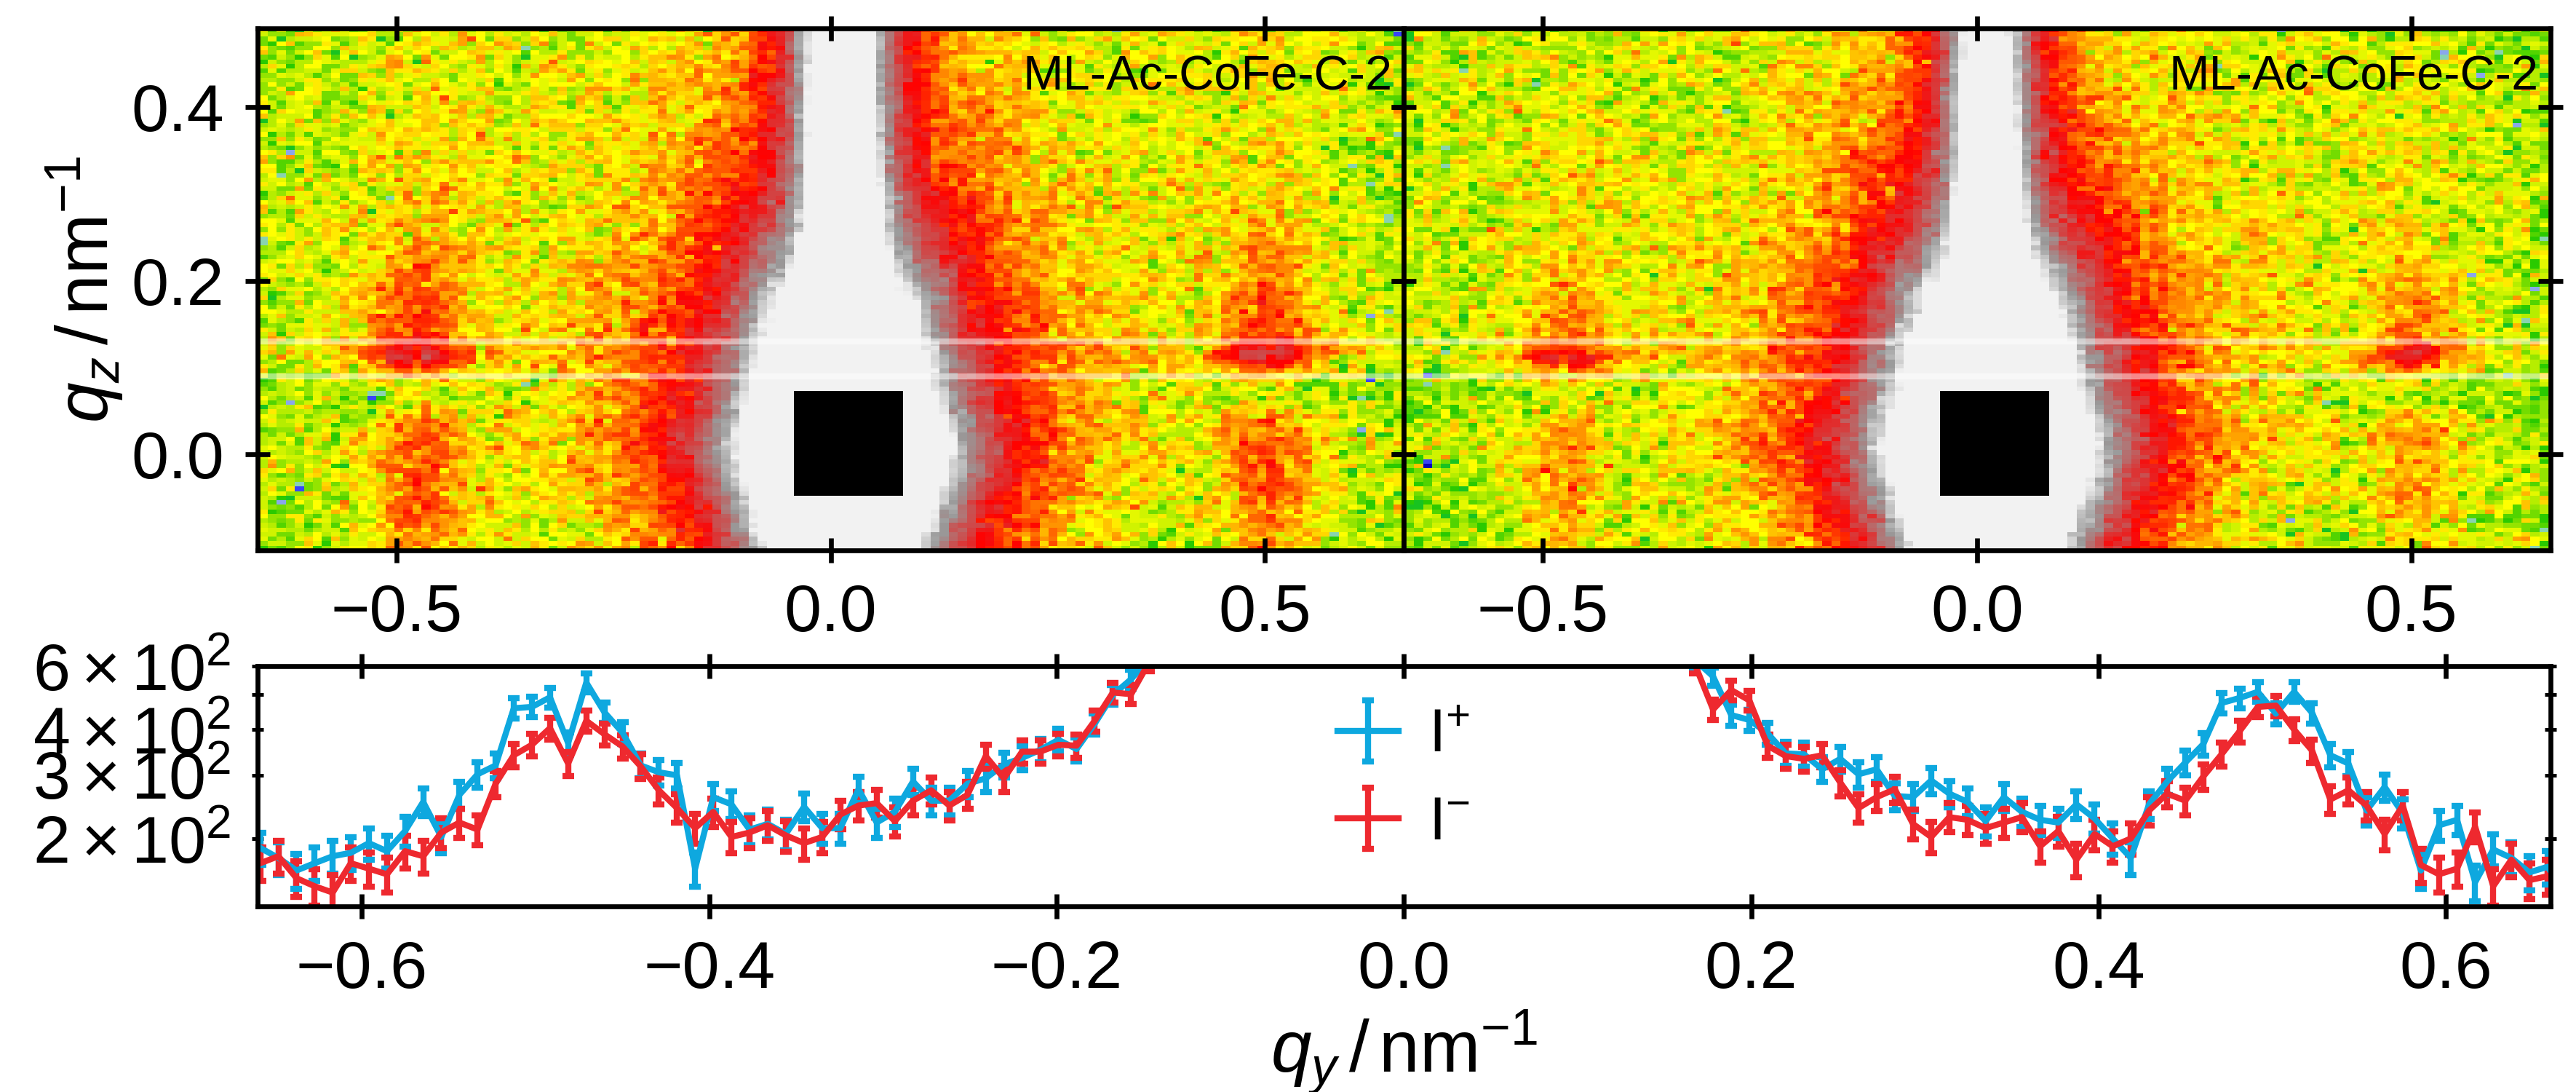
\includegraphics{monolayers_GISANS_ML-Ac-CoFe-C-2_ZFC5K_negField}
    \caption{\label{fig:monolayer:magneticStructure:negativeField}PolGISANS of ML-Ac-CoFe-C-2 after ZFC and saturation in a magnetic field of $4 \unit{T}$ measured in a negative magnetic field $-100 \unit{mT}$.}
  \end{figure}

\end{document}